\documentclass[11pt, spanish]{article}
\usepackage[utf8]{inputenc}
\usepackage{listings} 
\usepackage{graphicx}
\usepackage{amsfonts}
\usepackage[dvipsnames]{xcolor}
\usepackage[T1]{fontenc}
\usepackage{bigfoot}
\usepackage{amsmath}
\usepackage[numbered,framed]{matlab-prettifier}
\usepackage{caption}
\usepackage[figurename=Figura, tablename=Tabla, font={small,tt}]{caption}

\makeatletter
    \setlength\@fptop{0\p@}
\makeatother

\date{}

\usepackage{geometry}
 \geometry{
 a4paper,
 left=30mm,
 right=30mm,
 top=30mm,
 }

\lstset{
	style              = Matlab-editor,
  	basicstyle         = \mlttfamily,
  	escapechar         = ",
  	mlshowsectionrules = true,
	framesep=4.5mm,
	framexleftmargin=2.5mm,
	fillcolor=\color{White},
	rulecolor=\color{Black},
	numberstyle=\normalfont\tiny\color{Black}
}

\captionsetup[lstlisting]{font={small,tt}}
\renewcommand{\lstlistingname}{Script}

\newcommand\x{\times}
\newcommand\bigzero{\makebox(0,0){\text{\huge0}}}
\newcommand*{\bord}{\multicolumn{1}{c|}{}}
\newcommand{\norm}[1]{\left\lVert#1\right\rVert}


\begin{document}

\author{Sebastián Valencia Calderón \\ 201111578}
\title{Laboratorio 2: Solución de sistemas lineales en \textsc{MATLAB}}
\maketitle

%====================================================================

\section{Introducción}

Los sistemas de ecuaciones lineales aparecen en una gran variedad de aplicaciones en ciencia e ingeniería. La naturaleza algorítmica de las soluciones, da lugar a estudiar su eficiencia, su precisión y la representación de los algoritmos y los datos alrededor de ellas. Existen dos métodos para la soluciones de los sistemas de ecuaciones lineales, los iterativos y los no iterativos o directos. Ambos métodos, involucran pasos que pueden ser intensivos en el uso de recursos computacionales mas aun, si se trata de un sistema de grandes dimensiones. Los problemas fundamentales que pueden estudiarse están principalmente relacionados en las siguientes categorías:

\begin{enumerate}
\item Cuántas operaciones aritméticas son necesarias para aplicar un método propuesto.
\item Cuál va a ser la precisión o exactitud de la solución hallada por el método propuesto.
\item Cómo puede estimarse la precisión de los cálculos realizados.
\end{enumerate}

Sobre estas tres categorías, se plantean los principales problemas de la computación científica en relación con los problemas de solución de sistemas de ecuaciones lineales. Este tipo de problemas, se presentan de la siguiente manera: dado un sistema de la forma $A \times x = b$, donde $A$ es una matriz en $\mathbb{R}^{n \times m}$, y $b$ es un vector en $\mathbb{R}^{n}$, se desea hallar un vector en $\mathbb{R}^m$ que satisfaga la igualdad. De manera más formal, se busca responder a la pregunta de si el vector $b$ puede expresarse como un combinación lineal de los vectores columnas de la matriz.\\

En este caso en particular, se estudia la solución, eficiencia, y diseño de los procedimientos dispuestos en \textsc{MATLAB} para la solución de sistemas lineales. De igual forma, se explora la representación de las matrices y las características particulares que puedan mejorar la eficiencia de los procedimientos. A través de los experimentos realizados, se pretende cumplir los siguientes objetivos.

\begin{itemize}
\item Hacer uso y comprender la importancia de algunos métodos iterativos y no iterativos de solución de sistemas lineales disponibles en \textsc{MATLAB}.
\item Distinguir algunos sistemas lineales que por su estructura conviene resolverlos mediante métodos de solución de sistemas lineales específicos.
\item Identificar algunos casos que implican el mal condicionamiento de una matriz para ser resueltos mediante métodos iterativos o, por el contrario, por métodos no iterativos.
\end{itemize}

%==================================================================

\section{Procedimiento}


%==================================================================

\section{Resultados}

\subsection{Métodos iterativos}

\begin{enumerate}

%-----------------------------------------------------------------------------------------------------------------------

\item A continuación, se incluye una descripción de la función de \textsc{MATLAB} \texttt{linsolve()}, y unos breves ejemplos de su funcionamiento. La función \texttt{linsolve()}, la cual tiene dos parámetros \texttt{(A, B)}, tiene como objetivo solucionar el sistema de ecuaciones lineales de la forma $A \times x = b$. Es decir, en caso de que el sistema tenga solución, la función retorna el vector $x$ que satisface la igualdad mencionada. \textsc{MATLAB}, hace uso de optimizaciones dinámicas según las características de la matriz $A$. Si $A \in \mathbb{R}^{n\times n}$, entonces se usa la factorización $LU$ de la matriz $A$. De otra forma, la factorizacion $QR$ de la matriz $A$. Como restricciones, se debe cumplir que en número de filas de $A$ debe ser igual al número de filas de $b$. Si $A \in \mathbb{R}^{n \times m} \wedge b \in \mathbb{R}^m \Rightarrow x \in \mathbb{R}^n$. En caso de que el problema no esté bien definido, \textsc{MATLAB}, lanza una advertencia. La advertencia, se puede omitir asignando \texttt{linsolve(A, B)} a un vector de dos variables, donde la primera posición corresponde a la solución del problema y la segunda al recíproco del número de condición de $A$ de ser cuadrada, de lo contrario, el rango de $A$ (\texttt{[X, R] = linsolve(A, b)}).\\

A manera de ejemplo, se quiere resolver el sistema lineal mostrado a continuación. De manera algebraica, es posible demostrar que el sistema tiene solución y de hecho es $[2\ -3\ 4]$. \textsc{MATLAB}, es capaz de llegar a la misma respuesta haciendo uso de la función estudiada. Cabe resaltar la pertinencia del uso de computadores con sistemas lineales de gran dimensión.

$$\left(\begin{array}{ccc} 1 & 2 & 2\\ 1 & 3 & 3\\ 2 & 6 & 5 \end{array}\right) \hat{x} = \left(\begin{array}{c} 4\\ 5\\ 6 \end{array}\right)$$

Ahora, se quiere resolver el sistema lineal mostrado a continuación. De manera algebraica, es posible demostrar que el sistema tiene infinitas soluciones. Esto, por la teoría general del álgebra lineal. Para llegar a la misma conclusión a través de \textsc{MATLAB}, es necesario hacer uso de la función actualmente estudiada.

$$\left(\begin{array}{cccc} 1 & 2 & 0 & 1\\ 1 & 1 & 1 & -1\\ 3 & 1 & 5 & -7 \end{array}\right) \hat{x} = \left(\begin{array}{c} 7\\ 3\\ 1 \end{array}\right)$$

Al intentar calcular este valor, sin hacer uso de la asignación de este a un vector de dos posiciones, \textsc{MATLAB}, indica la advertencia anteriormente discutida. La advertencia, dice lo siguiente: \texttt{Warning: Rank deficient, rank = 2, tol =  6.34e-15}. Sin embargo, al realizar la asignación pertinente \texttt{[X, R] = linsolve(A, b)}, $X$  toma el valor de $[0\ 3.33\ 0\ 0.33]$, y $R$, toma el valor de 2, es decir, el rango de la matriz. Si se hacen las verificaciones, se observa que la respuesta del sistema es una aproximación muy buena a la solución numérica más no algebraica del problema. De igual manera ocurre si no se tienen soluciones. En el script \ref{lst:linearsystems}, se detalla la implementacion en \textsc{MATLAB} de los problemas propuestos para ilustrar el uso básico de la función \texttt{linsolve()}.

%---------------------------------------------------------------------------------------------------------

\item El parámetro opcional a la función anteriormente estudiada OPTS, proporciona la facilidad de hacerle saber a \textsc{MATLAB}, las características particulares de la matriz $A$. Es decir, dado que existe un grupo de matrices particulares para las cuales existen algoritmos de factorización o solución directa de los sistemas, es posible optimizar el proceso al contarle a \textsc{MATLAB} estas características. 

\item Las posibles características que permiten tales optimizaciones internas, descritas en el literal anterior, se describen a continuación.

\begin{itemize}

\item \textbf{UT} Matriz triangular superior. Una matriz es triangular superior si todos los elementos bajo su diagonal son iguales a cero.

$$ A = 
  \left(
    \begin{array}{ccccc}
    \x    & \x       & \x    & \x    & \x \\ 
     & \x       & \x    & \x    & \x \\ 
          &   & \x    & \x    & \x \\
          & \bigzero &  & \x    & \x \\ 
          &          &       &  & \x \\ 
  \end{array}\right) \Rightarrow \forall\ (i,\ j)\ ;\  i > j\ ;\ A_{i,j} = 0
$$

La solución un sistema de ecuaciones de las cuales las ecuaciones del lado izquierdo puedan representarse como matrices de esta forma, es mediante sustitución iterativa. Es decir, primero, se halla $x_n$, ya que el último pivote (el cual debe ser distinto de cero, por la suposición de que se tiene una solución), lleva de manera sencilla a encontrar este valor. Una vez se cuente con este valor, es sencillo encontrar $x_{n-1}$, y así de manera sucesiva hacia atrás.

\item \textbf{LT} Matriz triangular inferior

$$ A = 
  \left(
    \begin{array}{ccccc}
    \x &      &     &    &					\\
    \x & \x  &     &   \bigzero &              	\\
    \x & \x & \x &		&  	\\
    \x & \x & \x & \x &     			\\
    \x & \x & \x & \x & \x
  \end{array}\right) \Rightarrow \forall\ (i,\ j)\ ;\  i < j\ ;\ A_{i,j} = 0
$$

\item \textbf{SYM} Matriz simétrica real o compleja conjugada

$$A \in \mathbb{R}^{n \times m}\ ;\ A^T = A$$

\item \textbf{RECT} Matriz general rectangular

$$A \in \mathbb{R}^{n \times m}\ ;\ n \neq m$$

\item \textbf{POSDEF} Matriz positiva definida

$$A \in \mathbb{R}^{n \times n}\ ;\ \forall\ v \in \mathbb{R}^n\ ;\ v \neq 0\ v^{T}Av > 0$$

\item \textbf{UHESS} Matriz superior de Hessenberg

\[
\begin{bmatrix}
    x_{11}       & x_{12} & x_{13} & \dots & x_{1n} \\
    x_{21}       & x_{22} & x_{23} & \dots & x_{2n} \\
    \hdotsfor{5} \\
     0 & \dots       & x_{n, n-1} & \dots & x_{nn}
\end{bmatrix}
\]

\item \textbf{TRANSA} Matriz conjugada transpuesta, se refiere a si la función\texttt{linsolve()}, resuelve el sistema para la matriz transpuesta de la dada por argumento.

\end{itemize}

%------------------------------------------------------------------------------------------------------

\item Para generar las matrices aleatorias, se usa el script \ref{lst:randmatrix}, el cual, recibe las dimensiones de la matriz deseada y el tipo deseado, el último parámetro, puede ser de los siguientes tipos, los cuales representan lo mismo que en el literal anterior. \texttt{UT, LT, SYM, RECT, POSDEF, UHESS, TRANSA}. Para generar matrices del tipo \texttt{UT}, se hace uso de la función de \texttt{MATLAB} \texttt{triu}, al igual que \texttt{randi}. Para la generación de matrices tip \texttt{LT}, se usa la función \texttt{tril}. Para generar matrices del tipo \texttt{SYM}, se suman dos matrices haciendo uso de \texttt{triu}, las matrices rectangulares se generan directamente con la función \texttt{randi}. Para la matriz superior de Hessenberg, se hace uso de la función \texttt{hess}.\\

 Para la matriz de tipo \texttt{TRANSA}, se usó la función \texttt{complex} y \texttt{conj}. Por último, la matriz de tipo \texttt{POSDEF}, se genera a partir de una matriz diagonal estrictamente dominante, para las cuales se cumple que $|a_{ii}| > \sum_{j \neq i} |a_{ij}|\ \forall\ i,\ j = 1\ \dots n $. Se sabe que estas matrices son positivas definidas. Un procedimiento para generar este tipo de matrices, se encuentra en \cite{greenbaum2012numerical}, página 346, se adapta este algoritmo, y se genera de manera consistente cualquiera de estos tipos de algoritmos. Además de devolver la matriz adecuada según el tipo, el script \ref{lst:randmatrix} retorna un vector $b$ consistente con las dimensiones. A continuación se incluye un ejemplo de la ejecución de el script \ref{lst:randmatrix}, para cada tipo de matriz.

\begin{itemize}
\item \textbf{UT} \texttt{[mat, b] = randmatrix(4, 'UT')}

$$mat = \left(\begin{array}{cccc} 7 & 4 & 3 & 2\\ 0 & 6 & 10 & 3\\ 0 & 0 & 5 & 1\\ 0 & 0 & 0 & 7 \end{array}\right)\ ;\ b = \left(\begin{array}{c} 4\\ 8\\ 5\\ 1 \end{array}\right)$$\\

\item \textbf{LT} \texttt{[mat, b] = randmatrix(4, 'LT')}
 
 $$mat = \left(\begin{array}{cccc} 6 & 0 & 0 & 0\\ 8 & 6 & 0 & 0\\ 3 & 5 & 9 & 0\\ 2 & 7 & 5 & 3 \end{array}\right)\ ;\ b = \left(\begin{array}{c} 7\\ 7\\ 7\\ 10 \end{array}\right)$$\\
 
\item \textbf{SYM} \texttt{[mat, b] = randmatrix(4, 'SYM')}

$$mat =  \left(\begin{array}{cccc} 5 & 6 & 3 & 5\\ 6 & 8 & 2 & 5\\ 3 & 2 & 2 & 4\\ 5 & 5 & 4 & 8 \end{array}\right);\ b = \left(\begin{array}{c} 4\\ 2\\ 10\\ 7 \end{array}\right)
$$\\

Un test para esta matriz, es \texttt{issymmetric(mat)}.\\

\item \textbf{RECT} \texttt{[mat, b] = randmatrix(4, 'RECT')}

$$mat = \left(\begin{array}{cccccc} 35 & 24 & 50 & 26 & 7 & 4\\ 96 & 58 & 124 & 63 & 8 & 5\\ 95 & 70 & 135 & 71 & 5 & 3\\ 65 & 38 & 85 & 43 & 1 & 2 \end{array}\right)\ ;\ b = \left(\begin{array}{c} 7\\ 8\\ 10\\ 10 \end{array}\right)
$$\\

El rango de esta matriz, siempre es el tamaño dado por parámetro al script \ref{lst:randmatrix}. Es decir, la matriz es de rango completo.\\

\item \textbf{POSDEF} \texttt{[mat, b] = randmatrix(4, 'POSDEF')}

$$mat = \left(\begin{array}{cccc} 64 & 4 & 4 & 8\\ 4 & 52 & 7 & 2\\ 9 & 8 & 104 & 9\\ 8 & 10 & 9 & 108 \end{array}\right)\ ;\ b = \left(\begin{array}{c} 9\\ 5\\ 9\\ 4 \end{array}\right)
$$\\

Un test para esta matriz, es \texttt{positivedefinite = all(eig(mat) > 0)}.\\

\item \textbf{UHESS} \texttt{[mat, b] = randmatrix(4, 'UHESS')}

$$mat =  \left(\begin{array}{cccc} 2 & -5 & -4 & -4\\ -13 & 11 & 5 & 0\\ 0 & 5 & 1 & 4\\ 0 & 0 & -3 & 2 \end{array}\right)\ ;\ b = \left(\begin{array}{c} 6\\ 9\\ 6\\ 2 \end{array}\right)
$$\\

\item \textbf{TRANSA} \texttt{[mat, b] = randmatrix(4, 'TRANSA')}

$$mat =  \left(\begin{array}{cccc} 6 + 8\, \mathrm{i} & 9 + 6\, \mathrm{i} & 9 + 3\, \mathrm{i} & 10 + 7\, \mathrm{i}\\ 1 + \mathrm{i} & 9 + 7\, \mathrm{i} & 7 + 7\, \mathrm{i} & 10 + 8\, \mathrm{i}\\ 6 + 9\, \mathrm{i} & 5 + 10\, \mathrm{i} & 9 + 8\, \mathrm{i} & 3 + 6\, \mathrm{i}\\ 5 + 10\, \mathrm{i} & 10 + 6\, \mathrm{i} & 6 + \mathrm{i} & 9 + 2\, \mathrm{i} \end{array}\right)\ ;\ b = \left(\begin{array}{c} 9\\ 6\\ 10\\ 7 \end{array}\right)
$$
\end{itemize}

%---------------------------------------------------------------------------------------------------------

\newpage

\item El script para crear las matrices, solucionar los sistemas usando \texttt{linsolve()}, y la medición de los tiempos, se incluye en el srcipt \ref{lst:linmeasurement}. Este script, arroja una matriz de medición para los sistemas con cada una de las opciones y una matriz de error con la misma configuración.\\

Como ejemplo, correr el comando \texttt{[M, E] = linmeasurement(5)}, arroja los siguientes resultados para la matriz de tiempos:



\begin{table}[h]
\centering
\resizebox{\columnwidth}{!}{%
\begin{tabular}{|l|c|c|c|c|c|c|c|}
\hline
&\textbf{UT}&\textbf{LT}&\textbf{SYM}&\textbf{RECT}&\textbf{POSDEF}&\textbf{UHESS}&\textbf{TRANSA}\\\hline
\textbf{UT}&0.005370081&0.000013210&0.002794560&0.000086133&-1.000000000&0.000021848&0.000070284\\\hline
\textbf{LT}&0.000016979&0.000005994&0.000026746&0.000016543&-1.000000000&0.000012827&0.000015403\\\hline
\textbf{SYM}&0.000007155&0.000005576&0.000015837&0.000012767&-1.000000000&0.000007909&0.000014417\\\hline
\textbf{RECT}&0.000007576&0.000005856&-1.000000000&0.000016461&-1.000000000&-1.000000000&-1.000000000\\\hline
\textbf{POSDEF}&-1.000000000&-1.000000000&0.000026553&-1.000000000&0.000111140&-1.000000000&0.000016571\\\hline
\textbf{UHESS}&0.000007460&0.000005317&0.000015736&0.000013214&-1.000000000&0.000008142&0.000014918\\\hline
\textbf{TRANSA}&0.000012907&0.000007945&0.000095468&0.000065643&-1.000000000&0.000013785&0.000100514\\\hline
\end{tabular}%
}
\end{table}

Ahora, se corre 10 veces el mismo experimento y se promedian los tiempos, los resultados se muestran a continuación:

\begin{figure}[htbp]
\centering
	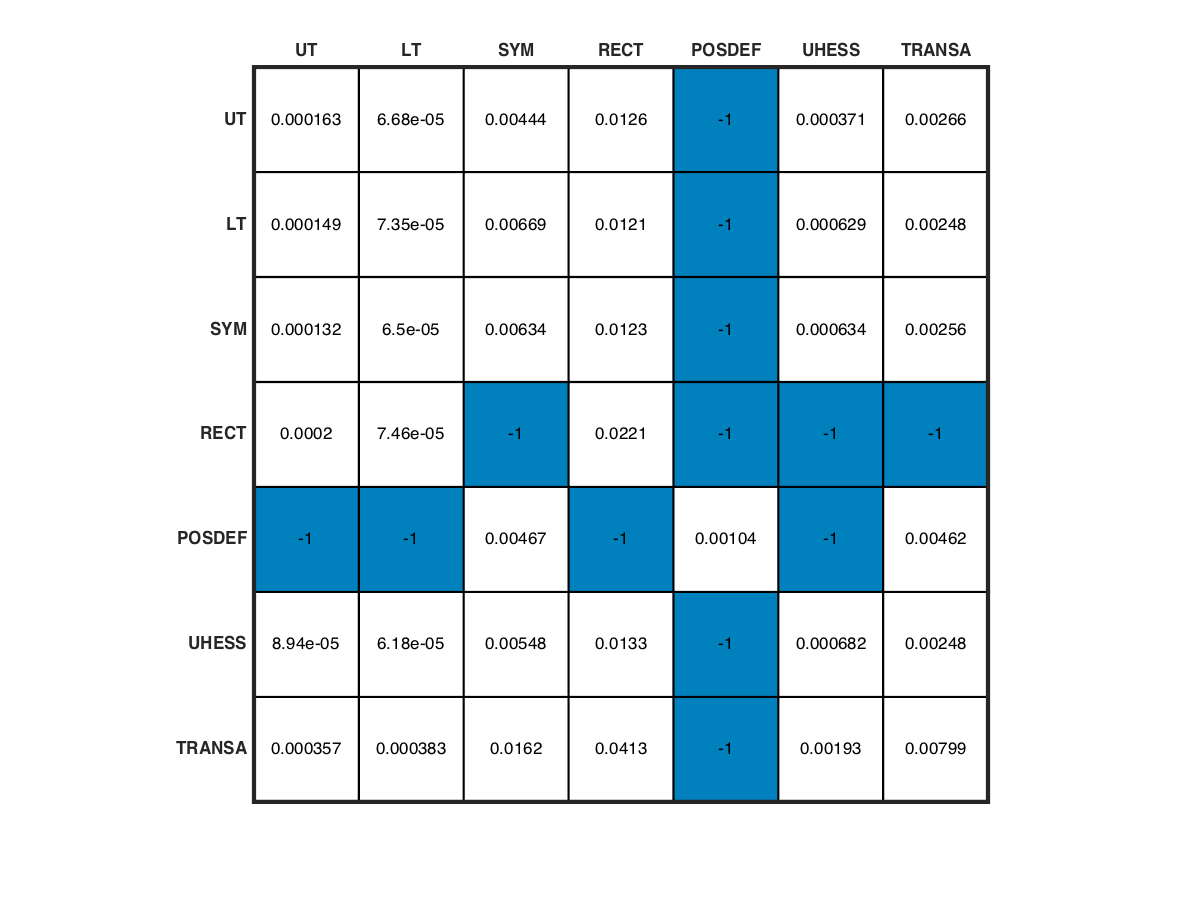
\includegraphics[scale=0.8]{data/img/plotlinear_times}
	\caption{Se muestra los tiempos requeridos para cada tipo de matriz y cada tipo de opción posible. Los menos uno, muestran los caso infactibles según las configuraciones de linsolve().}
\end{figure}

El proceso entero, se ejecuta mediante el script \ref{lst:runlinsolve}.

\newpage

\item Los tiempos de ejecución del algoritmo, son buenos en cada caso, sin embargo, no son concluyentes para evaluar la ejecución del algoritmo y las pertinencia de cada una de las posibles opciones. Es mejor confiar en el error de cálculo de cada uno de los métodos. Es decir, el error de calcular la solución de un sistema lineal con una configuración de \texttt{opts} dada, esto para cada matriz y para cada configuración.

\begin{figure}[h]
\centering
	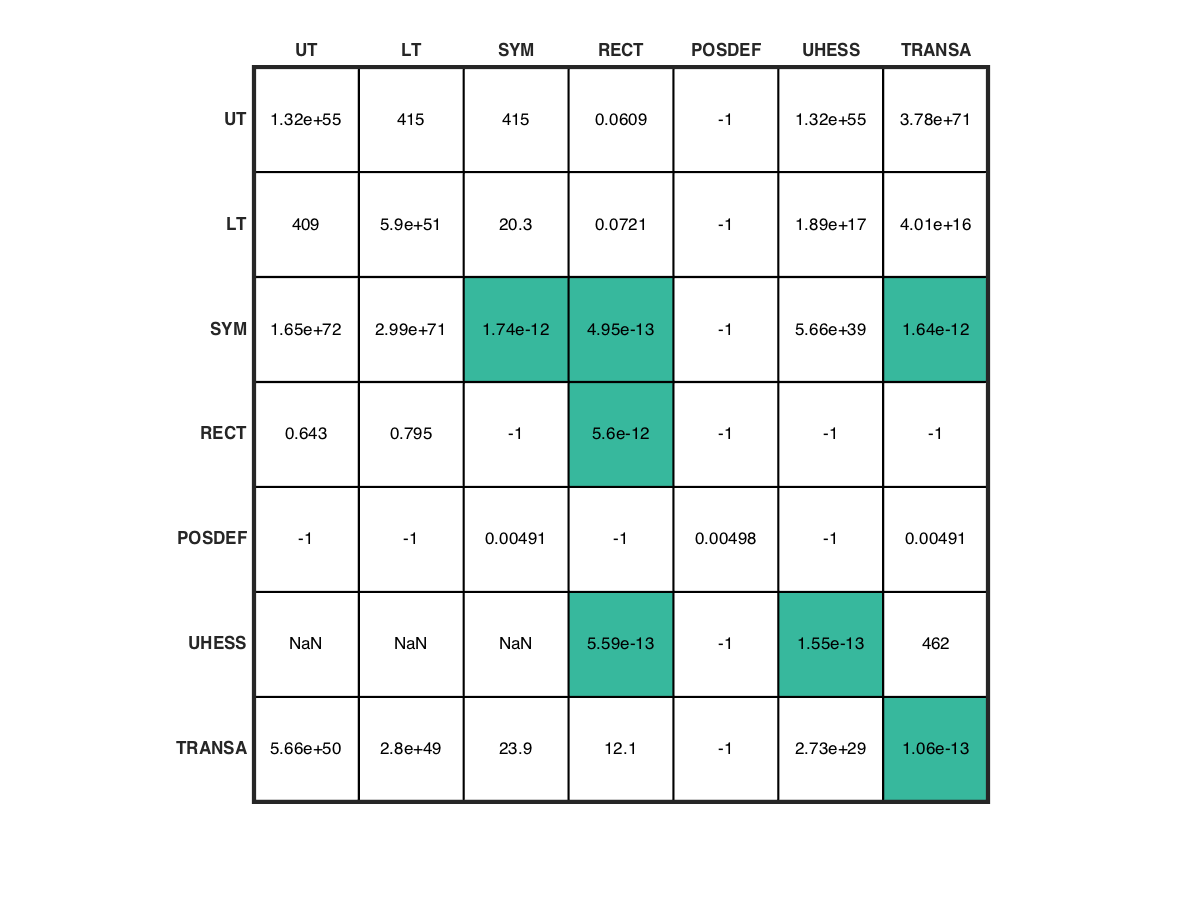
\includegraphics[scale=0.8]{data/img/plotlinear_error}
	\caption{Se muestra los errores de calculo para cada tipo de matriz y cada tipo de opción posible. Los valores resaltados, muestran los valores menores a una tolerancia dada, en este caso de $3\times 10 ^{-5}$.}
\end{figure}

Idealmente, solucionar una matriz de un tipo $\tau$, con la opción prendida para el mismo tipo $\tau$, debería arrojar los mejores resultados posibles. Es decir, es de fundamental importancia contar con errores bajos, sobre todo en la diagonal de la matriz de la anterior figura. Sin embargo, este no es el caso, por lo que se realiza un experimento para un tamaño menor de la matriz. El resultado, se evidencia en la figura siguiente. Como puede verse, se cumple el caso ideal, excepto para las matrices positivas definidas. Lo que puede resultar de esto, es que existe una perturbación demasiado considerable en las funciones de sustitución en \texttt{MATLAB}, este resultado, viene del hecho de que resolver matrices triangulares, trae un error mucho mayor a los otros tipos de matrices. Como puede verse en la figura anterior, resolver una matriz triangular con la opción \texttt{RECT}, es mucho mejor en términos de error que las opciones teóricamente ideales. Es fundamental resaltar que el tiempo ni es determinante sino el error de cálculo.

\begin{figure}[h]
\centering
	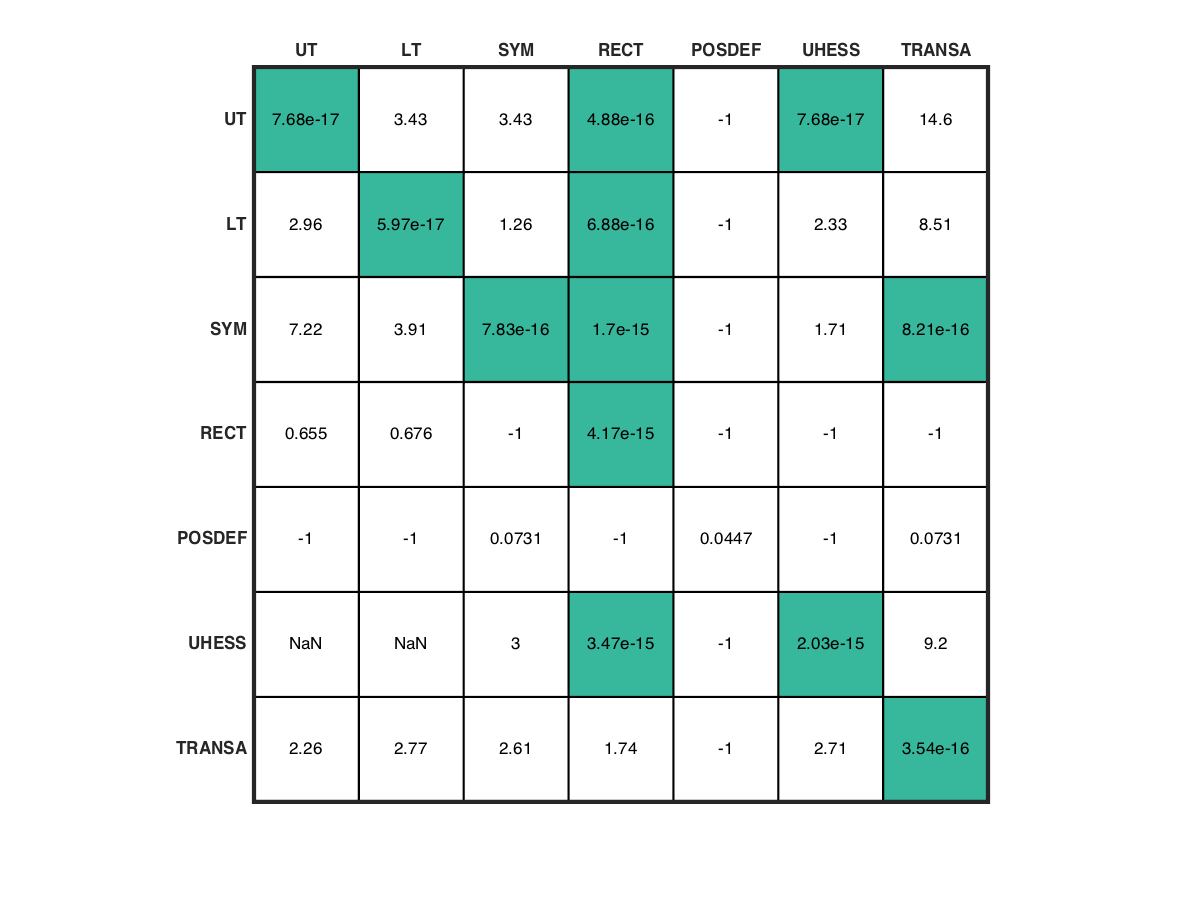
\includegraphics[scale=0.8]{data/img/plotlinear_errorsmall}
	\caption{Se muestra los errores de calculo para cada tipo de matriz y cada tipo de opción posible. Los valores resaltados, muestran los valores menores a una tolerancia dada, en este caso de $3\times 10 ^{-5}$. El tamaño de la matriz es mucho menor al anterior.}
\end{figure}

\end{enumerate}

\subsection{Métodos no iterativos}

\begin{enumerate}

\item La función \texttt{lsqr}, es una implementación en \texttt{MATLAB}, para los gradientes conjugados de ecuaciones normales. Esta función, intenta minimizar $\norm{b - Ax}$ para $x$, si $A$ es consistente, de tal manera que se resuelve el sistema de ecuaciones lineales $Ax = b$, de manera más específica, intenta solucionar mínimos cuadrados para la norma del residuo. Éste método iterativo, funciona mejor si $A$ es una matriz dispersa. La implementación, diseño y análisis de este método, se encuentra en la referencia \cite{Paige:1982:LAS:355984.355989}

$$x; Ax = b\ ;\ \min \norm{b - Ax}$$

Por otro lado, la función \texttt{symmlq}, intenta solucionar el sistema de ecuaciones lineales de la forma $Ax = b$, donde $A$ es una matriz simétrica cuadrada, no necesariamente positiva definida, esta debe ser de gran tamaño y dispersa.

\item Para la función \texttt{lsqr}, es deseable pero no requerido, una matriz dispersa. Para la función \texttt{symmlq}, es necesario una matriz simétrica.

\item Las matrices en el primer caso, pueden ser las anteriores, para el segundo caso, únicamente simétricas.

\item En le primer caso, se corre el script \ref{lst:runlsqr}, el cual hace uso del script \ref{lst:lsqrmeasurement}, para solucionar los sistemas de ecuaciones lineales. El único tipo de matriz solucionada por este función es positiva definida, pues se corrió de manera análoga al caso no iterativo, y ninguna matriz converge, excepto las positivas definidas, con un tiempo cercano a $0.00034$, con un error de $2.2\times 10^{-7}$. A continuación, se muestran los tiempos.

\begin{figure}[h]
\centering
	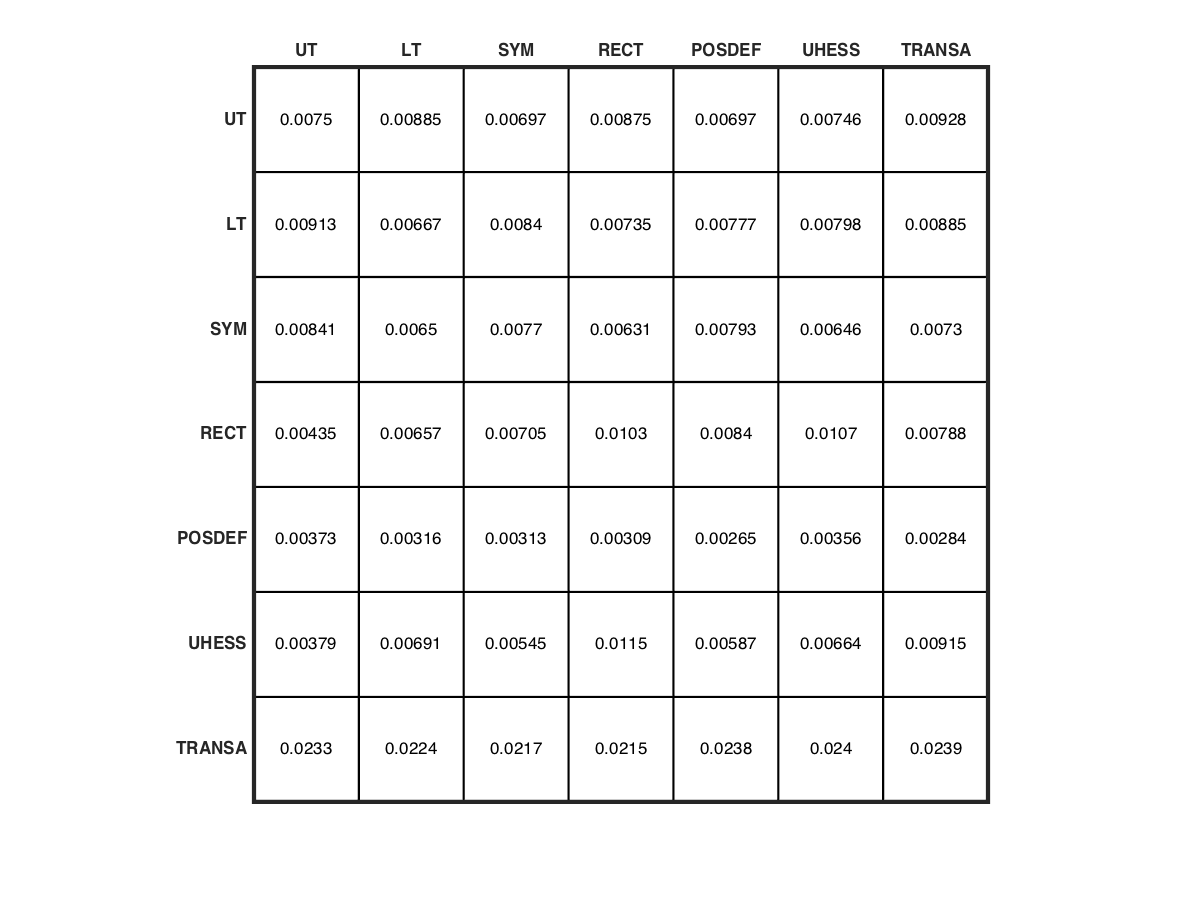
\includegraphics[scale=0.8]{data/img/plotlsqr_times}
	\caption{Se muestra los tiempos de cálculo para cada tipo de matriz haciendo uso de lsqr, aqui, se debe tener en cuenta que el tiempo incluye los valores independientemente de si la solución converge.}
\end{figure}

\newpage

\begin{figure}[h]
\centering
	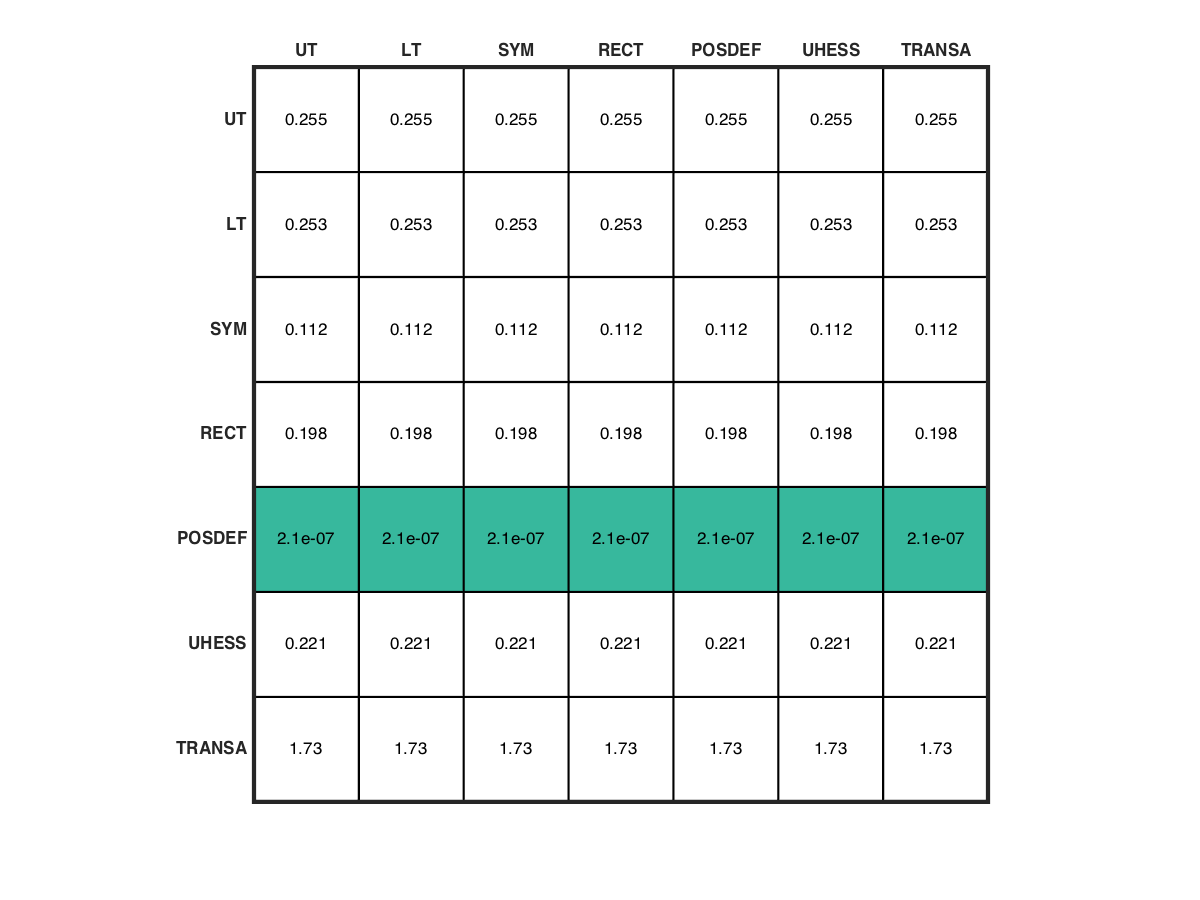
\includegraphics[scale=0.8]{data/img/plotlsqr_error}
	\caption{Se muestra los errores para cada tipo de matriz haciendo uso de lsqr, aqui, la solución sólo converge si la matriz es positiva definida, es decir, como se ve en los valores resaltados. La respuesta de MATLAB, es lsqr converged at iteration 6 to a solution with relative residual 2.2e-07.}
\end{figure}

En el caso de la función \texttt{symmlq}, donde la matriz debe ser simétrica, se realiza un experimento análogo haciendo uso de los scripts \ref{lst:runsymmlq} y \ref{lst:symmeasurement}. Los resultados, se muestran en las figuras 6 y 7.

\begin{figure}[h]
\centering
	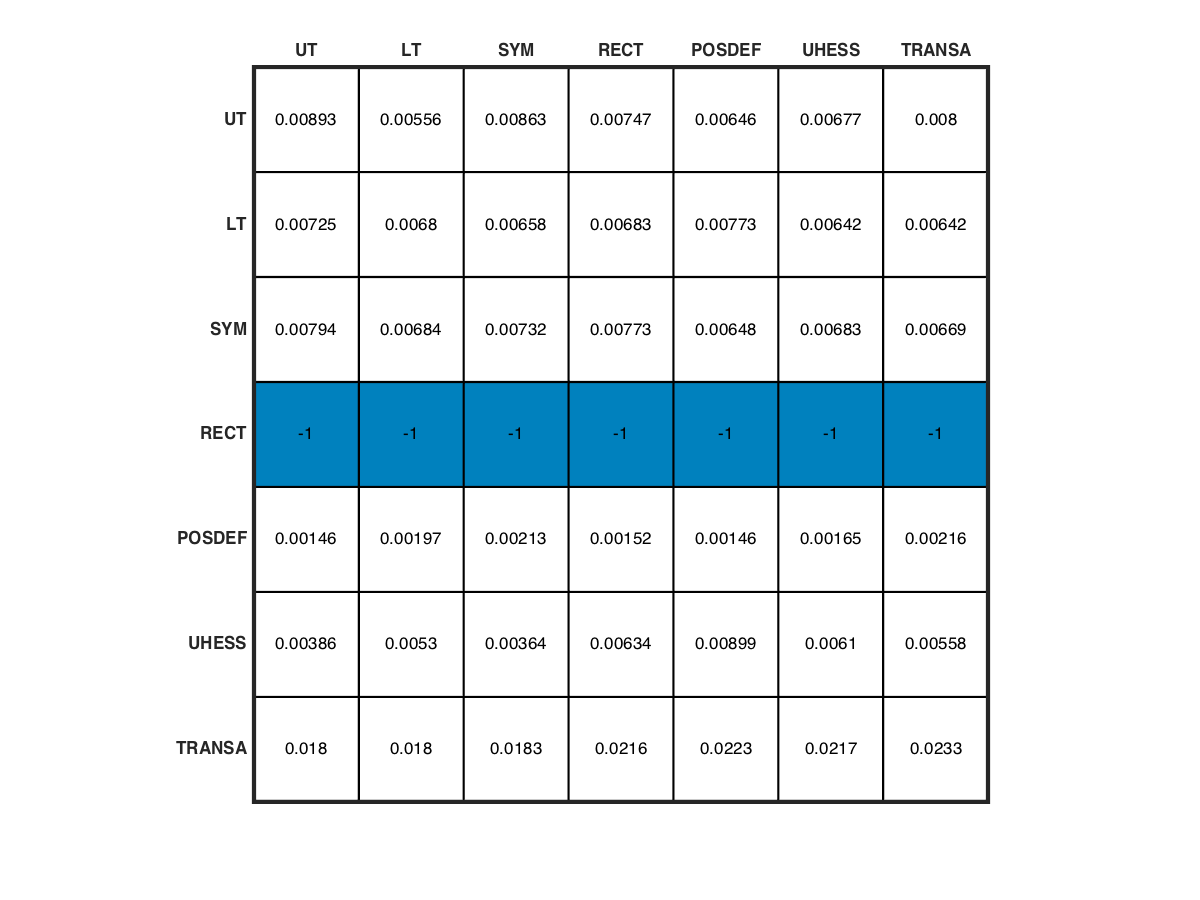
\includegraphics[scale=0.8]{data/img/plotsymmlq_times}
	\caption{Se muestra los tiempos de cálculo para cada tipo de matriz haciendo uso de symmlq, aqui, se debe tener en cuenta que el tiempo incluye los valores independientemente de si la solución converge. Los valores resultados, son infactibles.}
\end{figure}

\begin{figure}[h]
\centering
	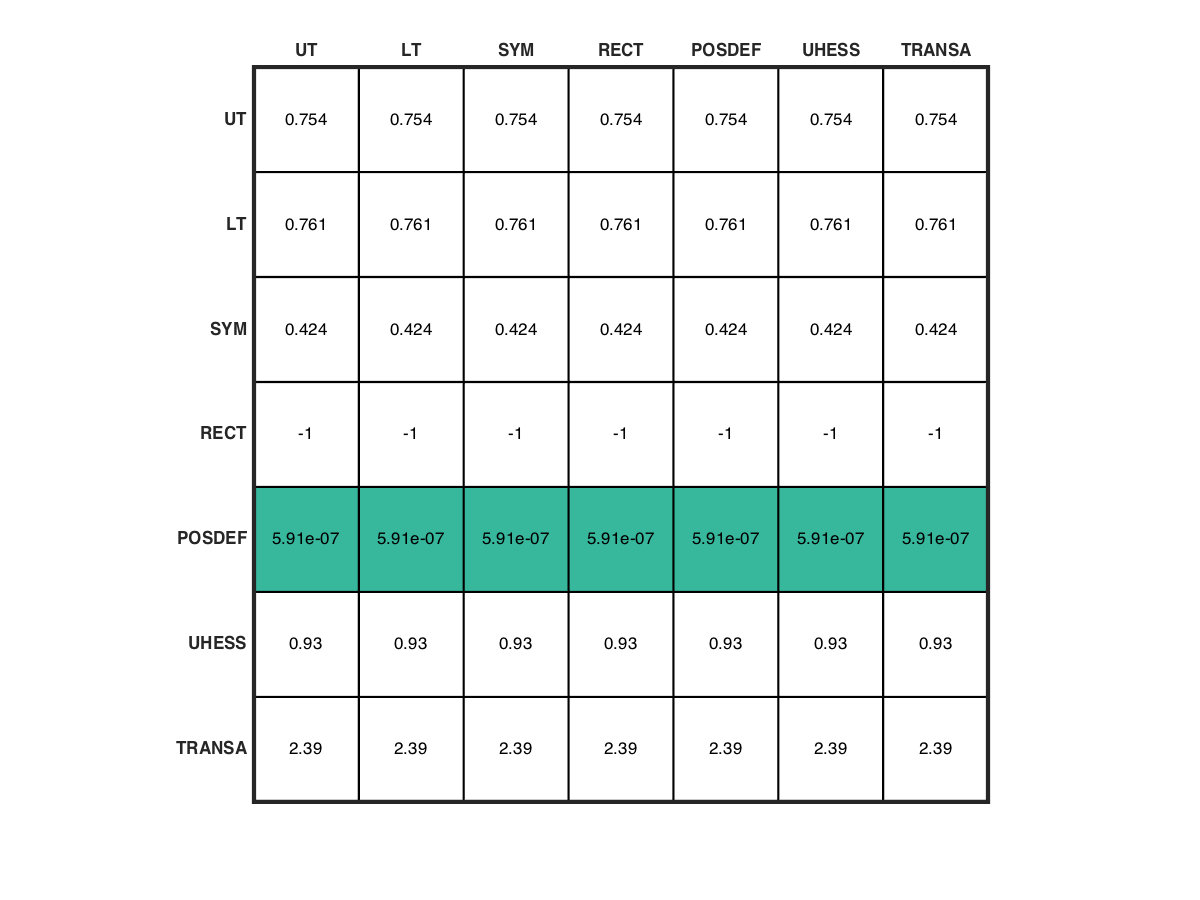
\includegraphics[scale=0.8]{data/img/plotsymmlq_error}
	\caption{Se muestra los errores para cada tipo de matriz haciendo uso de symmlq, aqui, la solución sólo converge si la matriz es positiva definida o simétrica, es decir, como se ve en los valores resaltados. La respuesta de MATLAB, es lsqr converged at iteration 6 to a solution with relative residual 5.91e-07.}
\end{figure}

Los valores únicamente convergen si las matices son o positivas definidas y en el segundo caso positivas definidas o simétricas, el tiempo de ejecución, es un poco mayor a los hallados con \texttt{linsolve}, lo que da lugar a pensar que en algunos casos, es mejor usar el mejor (el que minimice mejor error residual de la solución) método para resolver estos sistemas. De tal manera, se usarían los últimos dos métodos para resolver matrices positivas definidas, y el primero para las matrices simétricas, rectangulares, de Hessenberg y el caso traspuesto. El problema persistente, es el caso de las matrices triangulares, esto ultimo puede deberse a que el error se extiende por las divisiones sucesivas entre resultados anteriores, es decir la perturbación se debe al tamaño de los problemas.





\end{enumerate}

\newpage


%==================================================================

\section{Conclusiones}

Por medio del laboratorio, se pudo explorar el uso de las herramientas provistas por \textsc{MATLAB} para la solución de sistemas de ecuaciones lineales. Primero, un método que resuelve el sistema hallando la matriz inversa de $A$, para hallar la solución al sistema, dependiendo del tipo de la matriz, \textsc{MATLAB} realiza optimizaciones pertinentes para resolver el sistema de ecuaciones lineales usando las propiedades intrínsecas de la matriz $A$. Por otra parte, se hace uso de \textsc{LSQR} para resolver el mismo tipo de ecuaciones sobre matrices positivas definidas o simétricas. A través de los distintos experimentos, se pudo comprobar la perturbación total de la solución de cada incógnita y como esto afecta la solución global del sistema. Ademas, se comprobó que el tiempo no es determinante para soluciones numéricas, es mas importante contemplar el error y no el tiempo de ejecución. El tiempo puede considerarse, una vez se tenga certeza de una solución sin tanto error numérico.

\begin{itemize}
  \item Tener conciencia de la estructura, forma, características y propiedades de una matriz, es conveniente para determinar el mejor método para solucionar un sistema de ecuaciones lineales. La palabra mejor, se debe entender en el contexto de minimizar el error, de forma que el tiempo de computación y los recursos sean eficientes. Sin embargo, conviene concentrar el estudio en el error obtenido y no sobre el tiempo computacional invertido en solucionar el sistema.
  
   \item En experimentos posteriores, se puede incluir el estudio del acondicionamiento de las matrices y por lo tanto de las soluciones. Es necesario plantear una función general que estudie las propiedades de las matrices, y su condición para resolver de la mejor manera los sistemas lineales.
\end{itemize}

\newpage

%==================================================================

\section{Scripts}

\lstinputlisting[caption = {Uso de la funcion \texttt{linsolve()}, para los tres casos mas estudiados al resolver ecuaciones lineales. (\textbf{linearsystems.m})}, label={lst:linearsystems}]{data/scripts/linearsystems.m}

\lstinputlisting[caption = {Generación dinámica de matrices aleatorias del tipo triangular, simétrica, rectangular, positiva definida, superior de Hessenberg o una matriz compleja (\textbf{randmatrix.m})}, label={lst:randmatrix}]{data/scripts/randmatrix.m}

\newpage

\lstinputlisting[caption = {Experimento sobre distintos tipos de matrices y condiciones para el metodo \texttt{linsolve} (\textbf{linmeasurement.m})}, label={lst:linmeasurement}]{data/scripts/linmeasurement.m}

\lstinputlisting[caption = {Experimento completo para el caso de \texttt{linsolve}  (\textbf{runlinsolve.m})}, label={lst:runlinsolve}]{data/scripts/runlinsolve.m}

\lstinputlisting[caption = {Experimentación haciendo uso de \texttt{LSQR} (\textbf{runlsqr.m})}, label={lst:runlsqr}]{data/scripts/runlsqr.m}

\lstinputlisting[caption = {Experimentación haciendo uso de \texttt{LSQR} (\textbf{lsqrmeasurement.m})}, label={lst:lsqrmeasurement}]{data/scripts/lsqrmeasurement.m}

\lstinputlisting[caption = {Experimentación haciendo uso de \texttt{LSQR} simétrico (\textbf{runsymmlq.m})}, label={lst:runsymmlq}]{data/scripts/runsymmlq.m}

\lstinputlisting[caption = {Experimentación haciendo uso de \texttt{LSQR} simétrico. (\textbf{symmeasurement.m})}, label={lst:symmeasurement}]{data/scripts/symmeasurement.m}



\newpage

\addcontentsline{toc}{chapter}{\lstlistlistingname}
\lstlistoflistings

\bibliography{sample}

%=================================================================

\section{Bibliografía}

\begingroup
\renewcommand{\section}[2]{}%
\begin{thebibliography}{}

  \bibitem{greenbaum2012numerical} Greenbaum, A. and Chartier, T.P. {\em Numerical Methods: Design, Analysis, and Computer Implementation of Algorithms} 2012, Princeton University Press.
  
  \bibitem{Paige:1982:LAS:355984.355989} Paige, Christopher C. and Saunders, Michael A. {\em LSQR: An Algorithm for Sparse Linear Equations and Sparse Least Squares} March 1982, ACM Trans. Math. Softw..
  
\end{thebibliography}
\endgroup
\newpage

%==================================================================

\end{document}